\section{Versuchsaufbau und Messgeräte}
\subsection{AC-Suzeptibilität}
Für die Messung der AC-Suszeptibilität verwenden wir eine spezielle Schaltung, die sogenannte Hartshorn-Spulensystem. Dieses besteht aus einer Primärspule mit 2116 Windungen, welche von einem Wechselstrom durchflossen wird. Das von ihr erzeugte Magnetfeld induziert in zwei Sekundärspulen mit der gleichen Windungszahl wiederum einen Strom, welcher sich aufgrund des entgegengesetzten Windungssinns im nachgeschalteten OPV und Spannungsmessgerät aufhebt. Der Aufbau ist in Abbildung \ref{aufbau-AC} nochmals dargestellt. Bringt man nun in eine der beiden Spulen ein magnetisches Material, ändert sich die Flussdichte in der entsprechenden Spulen und das Messsignal ist ungleich null, welches von der Änderung der Magnetisierung mit dem Magnetfeld H, also von $\frac{\partial M}{\partial H}$ abhängt.


\begin{figure}[h!]
	\centering
	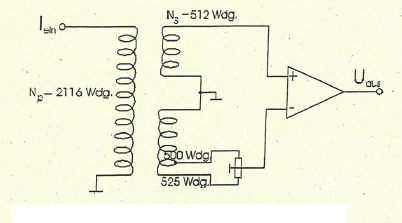
\includegraphics[height=8cm]{AC-auf.png}	
	~ %
	\caption{Hartshorn-Spulensystem für Messung der AC-Suszeptibilität \cite{Anleitung}}
	\label{aufbau-AC}
\end{figure}

\subsection{Phasenübergang der Indiumprobe}
Die Probe befindet sich auf einer Messapparatur in einem aufwändigen Kryostat mit fünf Glasschichten, die von außen nach Innen trennen: Luft ($T=300$K), Vakuum (thermische Isolation), Stickstoff ($T=75$K), Vakuum, Helium ($T=4,2$K), vgl. hierzu Abbildung \ref{aufbau}.

\begin{figure}[h!]
	\centering
	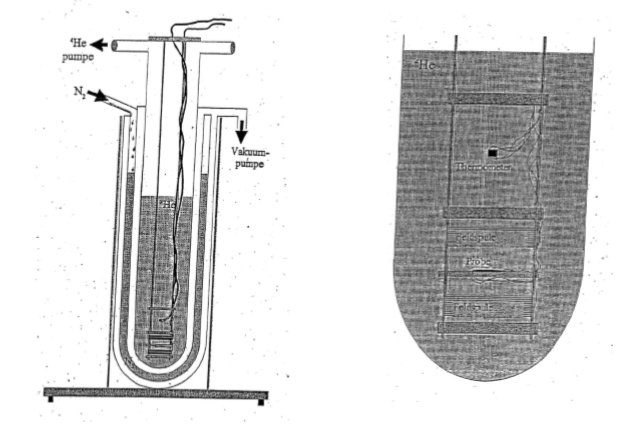
\includegraphics[height=8cm]{Aufbau.png}	
	~ %
	\caption{Messaufbau Phasenübergang Indium-Probe. \cite{Anleitung}}
	\label{aufbau}
\end{figure}

Für Indium gilt erfahrungsgemäß etwa $T_c=3,41$K, was sich unterhalb der Siedetemperatur von Helium befindet. Durch Reduktion des Drucks im Behälter sinkt auch die Siedetemperatur (vgl. Dampfdruckkurve), sodass wir auch Temperaturen unterhalb des klassischen Siedepunkts von Helium erreichen können. So ist es möglich, durch bloßes Öffnen und Schließen der Ventile den Temperaturbereich von $T$=2 bis $T$=4K zu durchfahren. Die Messung des Widerstands geschieht dabei über eine sog. 4-Punkt-Messung, bei der die Probe über vier Messpunkte kontaktiert wird. Dabei wird über zwei Spitzen eine Wechselspannung angelegt, während die anderen beiden Spitzen zur Messung des Spannungsabfalls in der Probe verwendet werden. Diese Methode bietet eine sehr hohe Messgenauigkeit, da die Messleitungen selbst keinen Strom tragen. Über einen Lock-In-Verstärker mit gespeicherter Eichkurve werden dabei ständig Messwerte aufgenommen und direkt in ein R-T-Diagramm aufgetragen. Der Lock-In-Verstärker stellt dabei einen sehr engen Bandpassfilter dar, welcher mittels eines Referenzsignals speziell nach der angelegten Frequenz sucht und damit Störsignale quasi ausschließt. Da der Widerstand der Probe in der supraleitenden Phase sehr gering ist, ist eine solche Methode zur Widerstandsmessung unabdingbar. Der Prozess geschieht weiterhin hinreichend langsam, als dass das System im ständigen Gleichgewicht betrachtet werden kann.
